%%
%% This is file `sample-acmlarge.tex',
%% generated with the docstrip utility.
%%
%% The original source files were:
%%
%% samples.dtx  (with options: `acmlarge')
%% 
%% IMPORTANT NOTICE:
%% 
%% For the copyright see the source file.
%% 
%% Any modified versions of this file must be renamed
%% with new filenames distinct from sample-acmlarge.tex.
%% 
%% For distribution of the original source see the terms
%% for copying and modification in the file samples.dtx.
%% 
%% This generated file may be distributed as long as the
%% original source files, as listed above, are part of the
%% same distribution. (The sources need not necessarily be
%% in the same archive or directory.)
%%
%% The first command in your LaTeX source must be the \documentclass command.
\documentclass[acmsmall, anonymous, review]{acmart}
%% NOTE that a single column version is required for 
%% submission and peer review. This can be done by changing
%% the \doucmentclass[...]{acmart} in this template to 
%% \documentclass[manuscript,screen,review]{acmart}
%% 
%% To ensure 100% compatibility, please check the white list of
%% approved LaTeX packages to be used with the Master Article Template at
%% https://www.acm.org/publications/taps/whitelist-of-latex-packages 
%% before creating your document. The white list page provides 
%% information on how to submit additional LaTeX packages for 
%% review and adoption.
%% Fonts used in the template cannot be substituted; margin 
%% adjustments are not allowed.
%%
%% \BibTeX command to typeset BibTeX logo in the docs
\AtBeginDocument{%
  \providecommand\BibTeX{{%
    \normalfont B\kern-0.5em{\scshape i\kern-0.25em b}\kern-0.8em\TeX}}}

%% Rights management information.  This information is sent to you
%% when you complete the rights form.  These commands have SAMPLE
%% values in them; it is your responsibility as an author to replace
%% the commands and values with those provided to you when you
%% complete the rights form.
\setcopyright{acmcopyright}
\copyrightyear{}
\acmYear{}
\acmDOI{}


%%
%% These commands are for a JOURNAL article.
%\acmJournal{}
%\acmVolume{}
%\acmNumber{}
%\acmArticle{}
%\acmMonth{}

%%
%% Submission ID.
%% Use this when submitting an article to a sponsored event. You'll
%% receive a unique submission ID from the organizers
%% of the event, and this ID should be used as the parameter to this command.
%%\acmSubmissionID{123-A56-BU3}

%%
%% The majority of ACM publications use numbered citations and
%% references.  The command \citestyle{authoryear} switches to the
%% "author year" style.
%%
%% If you are preparing content for an event
%% sponsored by ACM SIGGRAPH, you must use the "author year" style of
%% citations and references.
%% Uncommenting
%% the next command will enable that style.
%%\citestyle{acmauthoryear}

\usepackage{todonotes}
\usepackage{xspace}
\usepackage{listings}
\usepackage[all]{xy}


\newcommand{\todonote}[1]{\todo[inline, color=blue!20]{\textbf{TODO:} #1}}
\newcommand{\sectionword}{section}
\newcommand{\appendixword}{appendix}
\newcommand{\figureword}{Fig.}
\newcommand{\eqdef}{\overset{\mathrm{def}}{=}}
\newcommand{\ruleno}[1]{\mbox{[\textsc{#1}]}}
\newcommand{\bigslant}[2]{{\raisebox{.2em}{$#1$}\left/\raisebox{-.2em}{$#2$}\right.}}

\newcommand{\substupd}[3]{#1[#2 \mapsto #3]}

\newcommand{\taskst}[2]{\langle #1 ,\, #2 \rangle}
\newcommand{\mkenv}[2]{(#1 ,\, #2)}
\newcommand{\unigoal}[2]{#1 \equiv #2}
\newcommand{\conjgoal}[2]{#1 \land #2}
\newcommand{\disjgoal}[2]{#1 \lor #2}
\newcommand{\freshgoal}[2]{\texttt{\underline {fresh}} \, #1\;.\; #2}
\newcommand{\invokegoal}[3]{#1\,(#2, \, \dots, \, #3)}

\newcommand{\lazystream}[1]{\texttt{Lazy [{#1}]}}
\newcommand{\consstream}[2]{\texttt{Cons #1 [{#2}]}}

\newcommand{\tra}[1]{\mathcal{T}r^{ans}(#1)}
\newcommand{\trs}[1]{\mathcal{T}r^{st}(#1)}

\newcommand{\expranalog}[1]{E(#1)}

\newcommand{\mK}{\textsc{miniKanren}\xspace}

\newcommand{\lookuptime}[1]{\texttt{lookup}\,(#1)}
\newcommand{\addtime}[1]{\texttt{add}\,(#1)}
\renewcommand{\O}{\mathcal{O}}


%% Listings

\lstdefinelanguage{minikanren}{
keywords={fresh},
sensitive=true,
commentstyle=\small\itshape\ttfamily,
keywordstyle=\textbf,
identifierstyle=\ttfamily,
basewidth={0.5em,0.5em},
columns=fixed,
fontadjust=true,
literate={fun}{{$\lambda\;\;$}}1 {->}{{$\to$}}3 {===}{{$\,\equiv\,$}}1 {=/=}{{$\not\equiv$}}1 {|>}{{$\triangleright$}}3 {/\\}{{$\wedge$}}2 {\\/}{{$\vee$}}2,
morecomment=[s]{(*}{*)}
}

\lstset{
mathescape=true,
language=minikanren
}

\usepackage{letltxmacro}
\newcommand*{\SavedLstInline}{}
\LetLtxMacro\SavedLstInline\lstinline
\DeclareRobustCommand*{\lstinline}{%
  \ifmmode
    \let\SavedBGroup\bgroup
    \def\bgroup{%
      \let\bgroup\SavedBGroup
      \hbox\bgroup
    }%
  \fi
  \SavedLstInline
}


%%
%% end of the preamble, start of the body of the document source.
\begin{document}

%%
%% The "title" command has an optional parameter,
%% allowing the author to define a "short title" to be used in page headers.
\title{A Complexity Study for Interleaving Search}

%%
%% The "author" command and its associated commands are used to define
%% the authors and their affiliations.
%% Of note is the shared affiliation of the first two authors, and the
%% "authornote" and "authornotemark" commands
%% used to denote shared contribution to the research.
\author{Dmitry Rozplokhas}
\email{rozplokhas@gmail.com}
\author{Dmitry Boulytchev}
\email{dboulytchev@math.spbu.ru}
\affiliation{%
  \institution{Saint Petersburg State University and JetBrains Research}
  \country{Russia}
}

%%
%% By default, the full list of authors will be used in the page
%% headers. Often, this list is too long, and will overlap
%% other information printed in the page headers. This command allows
%% the author to define a more concise list
%% of authors' names for this purpose.
%\renewcommand{\shortauthors}{Trovato and Tobin, et al.}

%%
%% The abstract is a short summary of the work to be presented in the
%% article.
\begin{abstract}
  We study the worst-case time complexity of programs in \mK. We propose a model that breaks the evaluation time in \mK into
  several parts and provides methods to estimate the complexity of these different parts. These methods can be combined into an approach for
  analyzing the complexity of recursive relations using the ideas originating from symbolic execution. Our approach puts a number of limitations
  on the program being analyzed but we show that is still practically applicable by applying it to a number of typical relations in \mK.
\end{abstract}

%%
%% The code below is generated by the tool at http://dl.acm.org/ccs.cfm.
%% Please copy and paste the code instead of the example below.
%%
\begin{CCSXML}
<ccs2012>
<concept>
<concept_id>10011007.10011006.10011008.10011009.10011015</concept_id>
<concept_desc>Software and its engineering~Constraint and logic languages</concept_desc>
<concept_significance>500</concept_significance>
</concept>
<concept>
<concept_id>10011007.10010940.10011003.10011002</concept_id>
<concept_desc>Software and its engineering~Software performance</concept_desc>
<concept_significance>500</concept_significance>
</concept>
</ccs2012>
\end{CCSXML}

\ccsdesc[500]{Software and its engineering~Constraint and logic languages}
\ccsdesc[500]{Software and its engineering~Software performance}

%%
%% Keywords. The author(s) should pick words that accurately describe
%% the work being presented. Separate the keywords with commas.
\keywords{miniKanren, time complexity, interleaving search, triangular substitution, symbolic execution}


%%
%% This command processes the author and affiliation and title
%% information and builds the first part of the formatted document.
\maketitle


\section{Introduction}

This paper deals with the problem of the worst-case time complexity estimations for relational programs in \mK. Despite its simple implementation, the search in \mK has a number of subtleties
affecting the performance which are hard to think about intuitively altogether. It is easy to overlook some of them and the behavior of the search in certain cases can be really surprising.

\begin{figure}[t]
\begin{tabular}{p{5cm}p{5cm}}
\begin{lstlisting}[basicstyle=\small]
   length$^o$ = fun a n ->
     ((a === Nil) /\ (n === O)) \/
     (fresh (h t n')
        (a === Cons (h, t)) /\
        (n === S (n')) /\
        (length$^o$ l' n'))
     )
\end{lstlisting} &
\begin{lstlisting}[basicstyle=\small]
   length$_d^o$ = fun a n ->
     ((a === Nil) /\ (n === O)) \/
     (fresh (h t n')
        (a === Cons (h, t)) /\
        (length$_d^o$ l' n') /\
        (n === S (n')))
     )
\end{lstlisting}
\end{tabular}
\caption{Example of two implementations of the length calculating relation}
\label{fig:length_implementations}
\end{figure}

\begin{figure}[t]
    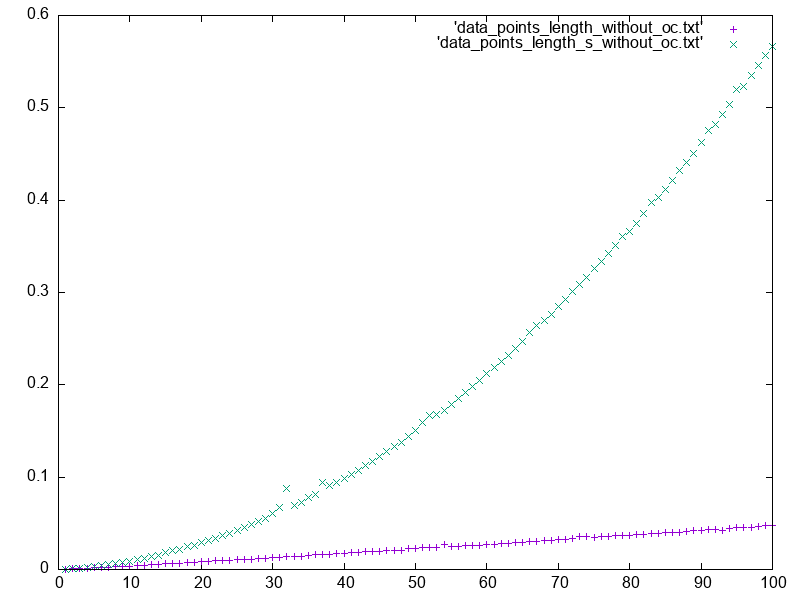
\includegraphics[width=6cm,height=5cm]{lengths_without_oc.png}
    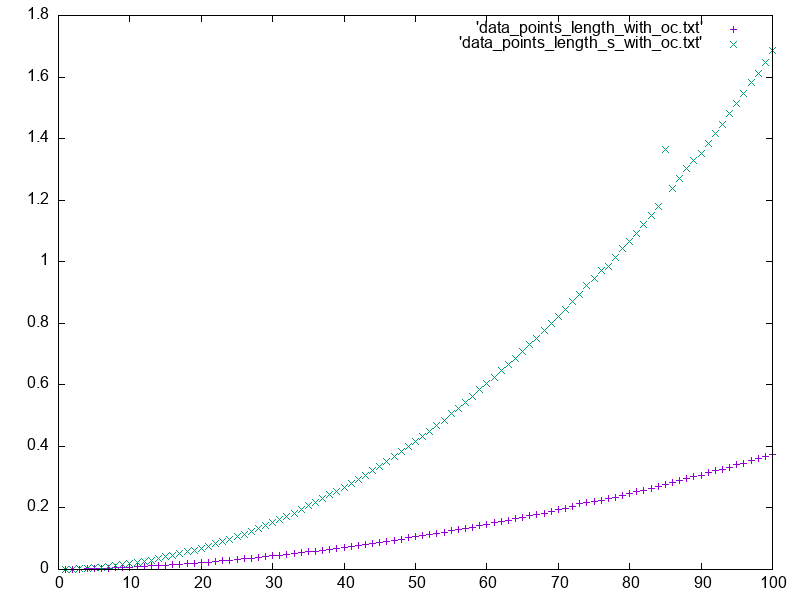
\includegraphics[width=6cm,height=5cm]{lengths_with_oc.png}
  \caption{Time of the search for the relations \lstinline|length$^o$| (purple) and \lstinline|length$_d^o$|} (green).
  Left: without occurs check.
  Right: with occurs check.
  \label{fig:length_plots}
\end{figure}

As a motivative example, consider two implementations of a standard recursive relation calculating the length of a list (see \figureword~\ref{fig:length_implementations}). They differ only in the
orders of conjuncts. Although the \lstinline|length$_d^o$| relation can be seen as a more direct definition of a function as a relation (all steps of usual length evaluation written up in order),
it is well-known that the \lstinline|length$^o$| with the recursive call in the end is much faster when running this relation backward (in fact, the search diverges if we
run \lstinline|length$_d^o$| backward, while for \lstinline|length$^o$| it terminates). What is less known and what we find more unexpected is the fact that if we run both relation
forward (specifying the list and asking for the length) \lstinline|length$^o$| is still much faster than \lstinline|length$_d^o$|, although they perform the same number of unifications
(actually during the evaluation of \lstinline|length$^o$| unified terms are even bigger). You can see the comparative time of the search in \figureword~\ref{fig:length_plots}. The difference is even
more staggering if we switch off occurs checks in unifications (for simple queries like this occurs checks never violated). In the same \figureword~\ref{fig:length_plots} you can see that
the \emph{asymptotic complexity} becomes different in this case: it is linear for \lstinline|length$^o$| and quadratic for \lstinline|length$_d^o$|.

After investigating the execution for this example in detail we found that the difference is caused not by unifications but by the process of \emph{scheduling} of goals during the search.
During the execution of a program in \mK a lazy structure is build that decomposes the goals into unifications, performs these unifications in a certain order and passes the results
appropriately. In our example this structure becomes linear in size just because of the order in conjunctions (when the recursive call is not the last) and increases the time of
scheduling significantly. This kind of effects is hard to predict and measure without a formal model for performance in \mK.

This paper presents such a model. We state that the total time of the search in \mK breaks into three separate parts: the time of scheduling ($T_s$) that breaks the evaluation into a sequence of
unifications, the time required to perform these unifications, and the time of reifications ($T_r$) that reconstruct the result in an expected form in the end. The time of unifications can be further
divided into the time of occurs checks ($T_{occ}$) during the unification and the time ($T_{uni}$) of the rest of the unification algorithm (this division will help us to see how large
is the part of the total time that occurs check, which often can be ommited, takes). So the total time of the search can be calculated as the sum of four components:

\[ T = T_s + T_{uni} + T_{occ} + T_r \]

We show how these components can be estimated and compared to each other in terms of asymptotics. The scheduling time complexity can be measured precisely since we link it to a specific value which we
call \emph{scheduling factor}, defined in terms of existing formal semantics of \mK (we recall the existing formal descriptions of \mK in \sectionword~\ref{sec:background}) and can be calculated using
a number of equations (\sectionword~\ref{sec:scheduling}). The other time components are hard to estimate precisely in general, as they are connected to the unification process, but we identify two
criteria that determine a wide range of cases for which these time components can be estimated easily (\sectionword~\ref{sec:uni-rei}). These separate methods for estimation of
different components of the time of the search can be put together in one approach calculating the time complexity for a given query to a recursive relation (if this query satisfies the stated
criteria) using the principles of symbolic execution (\sectionword~\ref{sec:symbolic}). We then show the applicability of our method by applying it for a number of realistic \mK relations (\sectionword~\ref{sec:evaluation}).

\section{Background: syntax and operational semantics}
\label{sec:background}

In this section we recollect some known formal descriptions for \mK language that will be used as a basis for our development.
Specifically, we restate the syntax of the basic version of the language and the operational semantics for program evaluation.
The descriptions here are taken from~\cite{CertifiedSemantics} (with a few non-essential adjustments for presentation purposes) to make
the paper self-contained, more details and explanations can be found there.

\begin{figure}[t]
\centering
\[
\begin{array}{ccll}
  \mathcal{C} & = & \{C_i^{k_i}\} & \mbox{constructors with arities} \\
  \mathcal{T}_X & = & X \cup \{C_i^{k_i} (t_1, \dots, t_{k_i}) \mid t_j\in\mathcal{T}_X\} & \mbox{terms over the set of variables $X$} \\
  \mathcal{D} & = & \mathcal{T}_\emptyset & \mbox{ground terms}\\
  \mathcal{X} & = & \{ x, y, z, \dots \} & \mbox{syntactic variables} \\
  \mathcal{A} & = & \{ x^?, y^?, z^? \dots \} & \mbox{logic variables} \\
  \mathcal{R} & = & \{ R_i^{k_i}\} &\mbox{relational symbols with arities} \\[2mm]
  \mathcal{G} & = & \mathcal{T_X}\equiv\mathcal{T_X}   &  \mbox{equality} \\
              &   & \mathcal{G}\wedge\mathcal{G}     & \mbox{conjunction} \\
              &   & \mathcal{G}\vee\mathcal{G}       &\mbox{disjunction} \\
              &   & \mbox{\lstinline|fresh|}\;\mathcal{X}\;.\;\mathcal{G} & \mbox{fresh variable introduction} \\
              &   & R_i^{k_i} (t_1,\dots,t_{k_i}),\;t_j\in\mathcal{T_X} & \mbox{relational symbol invocation} \\[2mm]
  \mathcal{S} & = & \{R_i^{k_i} = \lambda\;x_1^i\dots x_{k_i}^i\,.\, g_i;\}\; g & \mbox{specification}
\end{array}
\]
\caption{The syntax of \mK}
\label{fig:syntax}
\end{figure}

The syntax of the basic version of \mK is shown in Fig.~\ref{fig:syntax}. 
All data is presented using terms $\mathcal{T}_X$ built from a fixed set of constructors $\mathcal{C}$ with known arities and variables
from a given set $X$.
We parameterize the terms with an alphabet of variables since in the semantic description we will need \emph{two} kinds of variables:
\emph{syntactic} variables $\mathcal{X}$, used for bindings in the definition, and \emph{logic} variables $\mathcal{A}$, which are
introduced and unified during the evaluation.

In this version of \mK there are five types of goals: unification of two terms, conjunction and disjunction of goals (the
``\lstinline|conde|'' operator from the canonical versions of \mK, split in the ыtwo for simplicity), fresh logic variable introduction, and
invocation of some relational definition. For the sake of brevity, in code snippets we abbreviate immediately nested ``\lstinline|fresh|''
constructs into the one, writing ``\lstinline|fresh $x$ $y$ $\dots$ . $g$|'' instead of
``\lstinline|fresh $x$ . fresh $y$ . $\dots$ $g$|''.

The \emph{specification} $\mathcal{S}$ consists of a set of relational definitions and a top-level goal.
A top-level goal represents a search procedure which returns a stream of substitutions for the free variables of the goal.
The language we consider is first-order, as goals can not be passed as parameters, returned or constructed at runtime.

During the evaluation of \mK program an environment, consisting of a substitution for logic variables and a counter of allocated logic
variables, is threaded through computation and updated in every unification and fresh variable introduction.
The substitution in the environment at a given point and a given branch of evaluation contains all the information about relations between
the logical variables at this point, we will later refer to the substitution in the environment at a given point as a ``current substitution''
in informal explanations.
The different branches are combined via \emph{interleaving search} procedure~\cite{InterleavingSearch}.
The answers for the given query are extracted from the final environments (they are the values of the queried variables in the substitution
in the final environment).

This search procedure is formally described by an operational semantics in the form of a labeled transition system.
This semantics corresponds to the canonical implementation of interleaving search. 

\begin{figure}[t]
\centering
\[
\begin{array}{ccll}
  \Sigma & = & \mathcal{A} \to \mathcal{T}_\mathcal{A} & \mbox{substitutions} \\
  E & = & \Sigma \times \mathbb{N} & \mbox{environments} \\
  \\
  S & = & \taskst{\mathcal{G}}{E} & \mbox{task} \\
    &   & S \oplus S & \mbox{sum} \\
    &   & S \otimes \mathcal{G} & \mbox{product} \\
  \hat{S} & = & \diamond \; \mid \; S & \mbox{states} \\
  L & = & \circ \; \mid \; E & \mbox{labels} \\
\end{array}
\]
\caption{States and labels in the LTS for \mK}
\label{fig:operanional_semantics_states_labels}
\end{figure}

The form of states and labels in the transition system is defined in \figureword~\ref{fig:operanional_semantics_states_labels}.
Non-terminal states $S$ have a tree-like structure with intermediate nodes corresponding to partially-evaluated conjunctions
(``$\otimes$'') or disjunctions (``$\oplus$'').
A leaf in the form $\taskst{g}{e}$ determines a task to evaluate a goal $g$ in an environment $e$. For a conjunction node, its right child
is always a goal since it cannot be evaluated unless some result is provided by the left conjunct.
We also need a terminal state $\diamond$ to represent the end of the evaluation.
The label ``$\circ$'' is used to mark those steps which do not provide an answer; otherwise, a transition is labeled by an updated
environment.

\begin{figure*}
  \renewcommand{\arraystretch}{1.6}
  \[
  \begin{array}{cr}
    \taskst{t_1 \equiv t_2}{(\sigma, n)} \xrightarrow{\circ} \Diamond , \, \, \nexists\; mgu\,(t_1 \sigma, t_2 \sigma) &\ruleno{UnifyFail} \\
    \taskst{t_1 \equiv t_2}{(\sigma, n)} \xrightarrow{(mgu\,(t_1 \sigma, t_2 \sigma) \circ \sigma),\, n)} \Diamond & \ruleno{UnifySuccess} \\
    \taskst{g_1 \lor g_2}{e} \xrightarrow{\circ} \taskst{g_1}{e} \oplus \taskst{g_2}{e} & \ruleno{Disj} \\
    \taskst{g_1 \land g_2}{e} \xrightarrow{\circ} \taskst{g_1}{e} \otimes g_2 & \ruleno{Conj} \\
    \taskst{\mbox{\lstinline|fresh|}\, x\, .\, g}{(\sigma, n)} \xrightarrow{\circ} \taskst{g\,[\bigslant{\alpha_{n + 1}}{x}]}{( \sigma, n + 1)} & \ruleno{Fresh} \\
    \dfrac{R_i^{k_i}=\lambda\,x_1\dots x_{k_i}\,.\,g}{\taskst{R_i^{k_i}\,(t_1,\dots,t_{k_i})}{e} \xrightarrow{\circ} \taskst{g\,[\bigslant{t_1}{x_1}\dots\bigslant{t_{k_i}}{x_{k_i}}]}{e}} & \ruleno{Invoke}\\
    \dfrac{s_1 \xrightarrow{\circ} \Diamond}{(s_1 \oplus s_2) \xrightarrow{\circ} s_2} & \ruleno{DisjStop}\\
    \dfrac{s_1 \xrightarrow{e} \Diamond}{(s_1 \oplus s_2) \xrightarrow{e} s_2} & \ruleno{DisjStopAns}\\
    \dfrac{s \xrightarrow{\circ} \Diamond}{(s \otimes g) \xrightarrow{\circ} \Diamond} &\ruleno{ConjStop}\\
    \dfrac{s \xrightarrow{e} \Diamond}{(s \otimes g) \xrightarrow{\circ} \taskst{g}{e}}  & \ruleno{ConjStopAns}\\
    \dfrac{s_1 \xrightarrow{\circ} s'_1}{(s_1 \oplus s_2) \xrightarrow{\circ} (s_2 \oplus s'_1)} &\ruleno{DisjStep}\\
    \dfrac{s_1 \xrightarrow{e} s'_1}{(s_1 \oplus s_2) \xrightarrow{e} (s_2 \oplus s'_1)} &\ruleno{DisjStepAns}\\
    \dfrac{s \xrightarrow{\circ} s'}{(s \otimes g) \xrightarrow{\circ} (s' \otimes g)} &\ruleno{ConjStep}\\
    \dfrac{s \xrightarrow{e} s'}{(s \otimes g) \xrightarrow{\circ} (\taskst{g}{e} \oplus (s' \otimes g))} & \ruleno{ConjStepAns} 
  \end{array}
  \]
  \caption{Operational semantics of interleaving search}
  \label{fig:operanional_semantics_rules}
\end{figure*}

The transition rules are shown in Fig.~\ref{fig:operanional_semantics_rules}.
The introduced transition system is completely deterministic.
Therefore a derivation sequence for a state $s$ determines a certain \emph{trace}~--- a sequence of states and labeled transitions between
them.
It may be either finite (ending with the terminal state $\Diamond$) or infinite.
We will denote by $\trs{s}$ the sequence of states in the trace for initial state $s$ and by $\tra{s}$ the sequence of answers on
transitions in the trace for initial state $s$.
The sequence $\tra{s}$ corresponds to the stream of answers in the reference \mK implementations.

\section{Scheduling Complexity}
\label{sec:scheduling}

We may observe that the operational semantics described in the previous section can be used to calculate the number of elementary scheduling steps.
In this section we define a specific value which estimates the scheduling time and give some formulae to calculate this value for a given \emph{semantic
state}. However, our ultimate goal is to provide a way to deduce the complexity factor for a \emph{syntactic goal}. This problem will be addressed in
Section~\ref{which}, which will make use of recurrent formulae presented here.

We also restrict our considerations only by the case when the evaluation of a goal in question delivers a final number of answers. Indeed,
if the number of answers is infinite, no reasonable complexity estimation can be specified. A much more interesting question would be
the complexity estimation for coming up with some \emph{specific} answer; however for now this problem seems to be too hard to
tackle.

Our first idea is to take the number of states $d\,(s)$ in the \emph{finite} trace for a given state $s$:

\[ d\,(s) \; \eqdef \; | \trs{s} |  \]

However, it turns out, that this value alone in not enough to provide an accurate scheduling complexity estimation. The reason is that some
elementary steps in the semantics are not elementary in existing implementations. Namely, a careful analysis of the semantics discovers that
it involves a navigation to the leftmost leaf of the state, which in implementation corresponds to a number of
steps, proportional to the length of the leftmost branch of the state in question. Here we provide an \emph{ad-hoc} definition for this value, $t\,(s)$, and
assess its adequacy in Section~\ref{adequacy}:

\[
t\,(s) \eqdef \sum\limits_{s_i \in \trs{s}} lh\,(s_i) 
\]

where

\[
\begin{array}{rcl}
 lh\,(\taskst{g}{e})  &\eqdef& 1 \\
 lh\,(s_1 \oplus s_2) &\eqdef& lh\,(s_1) + 1 \\
 lh\,(s \otimes g)    &\eqdef& lh\,(s) + 1 \\
\end{array}
\]

\begin{lemma}
  For any state $s$

  \[
  d\,(s) \le t(s) \le d^2\,(s)
  \]
  
\end{lemma}

\begin{lemma}
  If

  \[\taskst{g}{e} \rightarrow s^\prime\]

  or

  \[\taskst{g}{e} \xrightarrow{a} s^\prime\]

  then

  \[d\,(\taskst{g}{e}) = d\,(s^\prime) + 1\]

  and

  \[t\,(\taskst{g}{e}) = t\,(s^\prime) + 1\]
\end{lemma}

\begin{lemma}
For any two states $s_1$ and $s_2$

\[
\begin{array}{rcl}
  d\,(s_1 \oplus s_2) &=& d\,(s_1) + d\,(s_2) \\
  d\,(s_1 \oplus s_2) &=& d\,(s_1) + d\,(s_2) + \min\,\{2\times d\,(s_1) - 1,\, 2\times d\,(s_2)\} 
\end{array}
\]

\end{lemma}

\begin{lemma}
For any state $s$ and any goal $g$

\[
\renewcommand{\arraystretch}{2}
\begin{array}{rclc}
  d\,(s \otimes g) &=& d\,(s)                                                      & + \\
                   & & \displaystyle\sum\limits_{a_i \in \tra{s}} d\,(\taskst{g}{a_i}) & \\
t\,(s \otimes g) &=& t\,(s) + d\,(s) + \displaystyle\sum\limits_{a_i \in \tra{s}} (t\,(\taskst{g}{a_i}) + \min\,\{2\times d\,(\taskst{g}{a_i}),\,2\times (d\,(s) - d_{a_i}\,(s) + \displaystyle\sum\limits_{j > i} d\,(\taskst{g}{a_j}))\} - 1) &
\end{array}
\]

where $d_{a_i}(s)$ is number of steps in the trace for state $s$ until the answer $a_i$ is produced.
\end{lemma}

The last exact equation is too cumbersome to use, so generally we will use some approximation of it. One option is to go with the fist argument of $\min$. It is a good approximation in a case when there are several answers passed to the second goal and there is none of them, scheduling time for which surpasses the scheduling time for all others combined.

\begin{corollary}
For any state $s$ and any goal $g$,
\[ t(s \otimes g) \le t(s) + d(s) +  \sum\limits_{a_i \in \tra{s}} (t(\taskst{g}{a_i}) + 2 d(\taskst{g}{a_i}). \]
\end{corollary}

In the case when there is only one answer, however, we should rather go with the second argument of $\min$.

\begin{corollary}
For any state $s$ and any goal $g$, if $\tra{s} = \{a_1\}$, then
\[ t(s \otimes g) \le t(s) + 3 d(s) + t(\taskst{g}{a_1}). \]
\end{corollary}

Finally, since we will calculate both metrics for some fixed program and we want an approximation up to a constant (which may depend on the structure of this program) we can derive a neat formulae for sequences of disjuncts and conjuncts that we will encounter.

\begin{lemma}

For $g = g_1 \lor \dots \lor g_k$ and any index $l$ from $1$ to $k$,

\[ \begin{array}{l}
d(\taskst{g}{e}) \le \sum\limits_{1 \le i \le k} d(\taskst{g_i}{e}), \\
t(\taskst{g}{e}) \le \sum\limits_{1 \le i \le k} t(\taskst{g_i}{e}) + k \sum\limits_{\begin{array}{c}1 \le i \le k \\ i \ne l\end{array}} d(\taskst{g_i}{e}).
\end{array} \]

\end{lemma}

\begin{lemma}

If $g = g_1 \land \dots \land g_k$ and if we denote by $A_i$ the set of all answers that are passed to $g_i$ at some stage if we start with some initial environment $e$:

\[ \begin{array}{l}
A_1 = \{ e \} \\
A_{i + 1} = \bigcup\limits_{a \in A_i} \tra{\taskst{g_i}{a}} \\
\end{array} \]

then

\[ \begin{array}{l}
d(\taskst{g}{e}) = \sum\limits_{1 \le i \le k} \;\; \sum\limits_{a \in A_i} d(\taskst{g_i}{a}), \\
t(\taskst{g}{e}) \le \sum\limits_{1 \le i \le k} \;\; \sum\limits_{a \in A_i} t(\taskst{g_i}{a}) + C(k) \sum\limits_{1 \le i \le k} \;\; \sum\limits_{a \in A_i} d(\taskst{g_i}{a}), \\
\end{array} \]

Where $C(k)$ is a constant depending only on $k$.

And in the case when all $A_i$ contain only one answer

\[ t(\taskst{g}{e}) \le \sum\limits_{1 \le i \le k} \;\; \sum\limits_{a \in A_i} t(\taskst{g_i}{a}) + C(k) \sum\limits_{1 \le i \le k - 1} \;\; \sum\limits_{a \in A_i} d(\taskst{g_i}{a}). \]

\end{lemma}

 \section{Unification and Reification Complexity}
\label{sec:uni-rei}

Syntactic unification of terms is a core operation for logic programming in whole and relational programming in particular.
However, the performance characteristics of conventional unification algorithms are rather hard to assess.
The known worst-case estimations say very little about the behaviour of unification in \emph{practically important cases}, and, in
general, the very notion of ``practical importance'' is hard to formalize (which constitutes a generic problem for applied complexity as well).

The practical observations witness, that while the worst-case complexity for the conventional unification algorithm is exponential, in the majority of
cases met in practical logic programming the time for each unification problem instance throughout the program execution is linear or even constant on the size of the input.

%So the inner workings of unification are often neglected when estimating performance of programs.

\mK has a distinctive way of implementing unification fitting in accordance with its ideology. First, since \mK aims at purely functional implementation of an embedded logical
language it uses a triangular form of substitution~\cite{UnificationTheory} which allows a simple extension in a non-mutable fashion. Such substitutions are lazy in the sense that
they hold a partially substituted value for each variable, so to obtain a fully substituted value it may be necessary to apply a substitution repeatedly. In particular, a full
cycle of substitution application is needed in the end of search to get the result for a queried variable. This process is called \emph{reification}. \mK uses the conventional Robinson's
algorithm for unification~\cite{RobinsonsAlgorithm}, adjusted for triangular substitutions~\cite{TRS}. Second, since \mK commits to adhere to logical consistency, by default it always
performs \emph{occurs checks} during the unification. Occurs check ensures that a binding being added into the substitution does not introduce any circularity, which is crucial for
establishing the soundness of unification results. However, being rarely violated, occurs check introduces a significant performance penalty, so some logical languages (such as \textsc{Prolog})
omit it.

In this section we show how the complexity of unification can be assessed for many practical cases. Specifically, we present two dynamic criteria
for relational programs, under which every unification (omitting occurs check) in the program performs a constant number of basic operations. At the same
time the occurs check, which complexity can be estimated separately, adds a significant overhead to the execution time and often increases the asymptotic complexity.
A number of programs satisfying given tests and showing the impact of occurs check are listed in \sectionword~\ref{sec:evaluation}.

The actual time of unification depends on a concrete choice for a data structure to represent triangular substitutions (which are, abstractly, maps from integers to terms).
Therefore we parameterize our estimations by two values~--- $\lookuptime{\sigma}$ and $\addtime{\sigma}$,~--- which represent, respectively, the
worst-case asymptotic complexity for lookup and add operations w.r.t. to a substitution $\sigma$. The obvious candidate data structure is standard library maps
for a host language (and many implementations like \textsc{miniKanren}-with-symbolic-constraints and \textsc{OCanren} follow this recipe), which have logarithmic complexity for both operations,
so we expect this multipliers to be negligible. However, some implementations like \textsc{microKanren} use associative lists for simplicity of presentation (which have linear-time
lookup and constant-time addition complexities) or more complex data structures like random-access lists (which have a log-time lookup and average constant-time addition complexities)
so we keep this parameterization for the general case. The review of performance of different date structures for triangular substitutions is given in~\cite{SubstDataStructs}.

The basic building block for the unification with triangular substitution is a \emph{walk} operation. This operation checks whether a given variable is mapped by a given substitution to a
term with a constructor at the top level. ``Walk'' continually looks up the substitution until a binding to a non-variable (in particular, no binding at all) is found. This
process can diverge only when there is a circular binding in the substitution, which, in turn, is exculded by the occurs check, so the substitutions are always consistent
in this sense~\cite{NominalUnificationWithTriangularSubstitutions}. Nevertheless ``walk'' can require a linear number (on the size of a substitution) of lookups.
However the variable-to-variable bindings occur rarely in practice and usually ``walk'' finds the required binding in one step. We can take the absence of variable-to-variable bindings
as our first criterion: for \emph{flat} substitutions (substitutions without such bindings) ``walk'' always makes only one lookup. We can relax this requirement by allowing a
constant number, independent on the inputs parameters of the topmost goal, of variable-to-variable bindings.

\begin{definition}
A substitution $\sigma$ is called \emph{constant-factor flat} if the number variable-to-variable bindings in $\sigma$ does not depend on the input parameters of the topmost goal.
\end{definition}

\begin{lemma}
If during the evalution of a goal all substitutions are constant-factor flat, then the time of any walk during that evaluation on substitution $\sigma$ is $\lookuptime{\sigma}$.
\end{lemma}

The unification of two terms goes by the standard recursive descent. Each time a variable is encountered in a term being unified a ``walk'' step is performed, and if it ends up with
an unbound varible the occurs check is performed and, if succeeded, the substitution is extended. As the substitution grows during the process  the unified terms grow,
too, and the descent can go beyond the size of initial terms. But we argue that this happens not that often. For example, for a linear case (when any variable occurs in unified terms at
most once) the extensions of the substitution during the unification do not affect the unification in other branches, so the recursion will stop at the minimal height of the terms. 

\begin{lemma}
  Given two terms $t_1$ and $t_2$ and a current constant-factor flat substitution $\sigma$, if any variable occurs at most once in at most one of the terms $\{t_1 \sigma, t_2 \sigma\}$,
  then the time this unification takes, excluding occurs checks, is $\O\,(\min\,\{|t_1 \sigma|, |t_2 \sigma|\}) \cdot (\lookuptime{\sigma} + \addtime{\sigma})$.
\end{lemma}

In particular, if the size of one of those two terms does not depend on the input parameters (which is usually the case) the unification performs a constant number of basic operation.
This is our second criterion: linearity and constant size of one the terms in every unification.

In the presence of occurs checks, however, we need to also go through every term we add in the substitution. This changes ``$\min$'' in the estimation above to ``$\max$'', making a huge
difference. Roughly speaking, in average the number of basic operations for every unification with occurs checks is approximately an average size of all terms unified in program
(which is usually linear of the input). Therefore occurs checks add a huge time overhead for program execution in \mK, both for asymptotics (see \sectionword~\ref{sec:evaluation})
and for observable time~\cite{WillThesis}. This fact calls for an investigation into ways of going around occurs checks in \mK. Although simply omitting them is not an option for \mK,
there are other known approaches (mostly explored for \textsc{Prolog}), for example static tests ensuring that occurs checks for a given program will never be violated~\cite{OccursCheckStaticTest}.
As far as we know, for now there are no such solutions adopted for \mK.

For now, as we estimate the time of every individual unification it might be not clear how it relates to the estimations for the scheduling time. But since we consider cases in which unification
is relatively fast (constant number of basic operations), the number of unifications during an execution plays more important role and it can be simply limited by the number of semantic
steps $d\,(s_{init}\,(input))$ (because every unification is a separate step in the semantics). Similarly, although the time of basic operations depends on the size of substitution in different points
of execution, logical variables for these bindings come either from the input (where there is usually a constant number of them) or from fresh variable allocations during the evalutation
(each of which is a a separate step in the semantics). So the number of allocated logic variables (and therefore the maximum possible number of bindings) is limited by

\[
FV\,(input) + d\,(s_{init}\,(input))
\]

So, for example, for a usual case, when our two criteria are satisfied and the input contains a constant number of logic variables, for a standard implementation and without occurs checks
the total time of unifications $T_{uni}$ is $\O\,(d\,(s_{init}\,(input))\cdot \log d\,(s_{init}\,(input)))$

The time of reification $T_r$ can be estimated in the same way, since reification simply goes through the resulting term similarly to occur check. So in the case when the resulting
substitution is constant-factor flat, the number of basic operations for the reification is limited by the size of the output (multiplied by a constant). This time is usually subdued by
the time of unification and scheduling, but not always (see examples in \sectionword~\ref{sec:evaluation}).



\section{Complexity Analysis via Symbolic Execution Schemes}
\label{sec:symbolic}

In the previous sections we presented some methods to estimate the time complexity for scheduling and unification/reification (for latter two only for some practical cases) in \mK, but they work
only for relational search in general, not for specific relational program. In this section we show how the latter task can be formulated and how those methods can be combined to solve
it using a notion of \emph{symbolic execution}.
Specifically, we add symbolic variables to \mK and use \emph{symbolic execution schemes} to build recursive inequalities for all components of our performance model.
These inequalities then can be be solved to provide a symbolic representation for asymptotic estimations.

The application of symbolic execution for time complexity analysis is well-known and was explored for logic programming in particular~\cite{SymbolicExecutionForAnalysis}.
Usually, symbolic execution graphs are used to capture all the details of program execution which are significant for performance and then the standard techniques for time (or other)
analysis of rewriting systems are applied. In contrast, we need a symbolic execution graphs only as a neat representation of a general scheme of a relational search for a
given program and then bring in performance details using \emph{ad hoc} methods described in the previous sections. So we use a restricted version of a graph that corresponds
precisely to a body of a relation, not unfolding any relational calls. For this reason we refer to them as ``symbolic execution schemes'' rather than ``symbolic execution graphs''.
This also means that we suppose that we know what answers any relational call in the program produces before we start the time complexity analysis.

\begin{figure}[t]
\begin{lstlisting}
   prefix$^o$ = fun n p ->
     (p === Nil) \/
     (fresh (n' pt pti)
        (n === S(n')) /\
        (prefix$^o$ n' pt) /\
        (incr-list$^o$ pt pti) /\
        (p === Cons(S(O), pti))
     )
\end{lstlisting}

\caption{Relational Prefixes Example}
\label{fig:prefixo_definition}
\end{figure}

To present the whole process in a clearer way we will go through it with a specific artificial example, in which almost all important details take place. The example is a relational program
for generating all prefixes of a list \lstinline|$[1,\dots,n]$| (with numbers represented in Peano encoding with constructors \lstinline|O| and \lstinline|S|). Consider the
following creative recursive solution: we either take an empty prefix or take any prefix for the same task for $n - 1$ (if $n > 0$), increment all the elements and add $1$ at the beginning.
The relation \lstinline|prefix$^o$| in \figureword~\ref{fig:prefixo_definition}, relating a number $n$ to some prefix $p$, follows this description directly. It uses a relation \lstinline|incr-list$^o$|
that increments all numbers in a given list, which implementation we do not include due to its straightforwardness. This relation provides required results: if we instantiate $n$ with some
Peano number and put a free logical variable for $p$ then $p$ will be bound to every prefix exactly once. It is an inefficient solution in many ways, but it is nice for presentation.

Now we want to estimate the time the search will take depending on a number we put as an input. To make our reasoning more precise we introduce the notion of \emph{symbolic variables}, which we will
denote with an overline ($\overline{a}, \overline{b}, \dots$) as opposed to the usual logic variables, which we will denote using a question mark ($a^{?}, b^{?}, \dots$). The symbolic
variables can be considered on two levels. At the level of symbolic execution each symbolic variable in \mK stands for some ground term (a term without logic variables inside), but we do not know which
term exactly. At the metalevel, where we reason about the complexity of a program, a symbolic variable $\overline{x}$ stands for a representation of some object $x$ from metatheory (it can be a number, a
string or a graph, for example) as a ground term, and we analyze how the program behaves depending on this object or some of its parameters. We will distinguish between these two levels throughout the
whole process of complexity analysis. For our example we consider the parametric query \lstinline{prefix$^o$ $\overline{k}$ $a^{?}$} with the first parameter instantiated by some number $k$
represented as a ground Peano term and second parameter left as a free logic variable, and ask how much time the search and its different stages will take depending on the value of $k$.

Our approach estimates the time complexity for some specific relational call with symbolic variables as arguments, not for a relation in general. We name every call we encounter to use these names in our
notations throughout the analysis (for example $pref = $ \lstinline{prefix$^o$ $\overline{k}$ $a^?$}). During the analysis we separately compute a number of factors for
the query that correspond to components of the overall time of the search in our model: the number of semantic steps $d^{pref}\,(k)$ and the scheduling factor $t_s^{pref}\,(k)$, which correspond to the number of semantic steps and the scheduling factor defined in \sectionword~\ref{sec:scheduling}, $t_{uni}^{pref}\,(k)$, which is the number of basic
operations performed during unifications in the execution of the call, exluding basic operations in occurs checks, $t_{occ}^{pref}(k)$, which is the number of basic operations performed during occurs checks, and $t_r^{pref}(k)$, which is the number of basic operations performed during the reification.

To achieve this, we build a symbolic execution scheme, mirroring the body of the examined relation, identify recursive calls and reconstructing recursive inequalities for all the aforementioned factors
by using the estimations described in the previous sections. 
We put a number of restrictions for the examined relational call for our approach (however, as can be seen from the
\sectionword~\ref{sec:evaluation}, the huge variety of real examples satisfy them): the two criteria from \sectionword~\ref{sec:uni-rei} should be satisfied (which we can check using the symbolic execution, too) to use estimates from that section, we also work only with relations in disjunctive normal form.

We need to know also two extra pieces of information to perform the analysis for a given call. First, to  know how to proceed after recursive calls we need to know the answers that the calls produce.
We describe them by sets of substitutions binding all the logical variables in the query to terms, possibly containing fresh logic variables and symbolic variables, the later we then specify in the metatheory (for example, $ANS^{pref}\,(k) = \{[a^? \gets \overline{p}] \mid \textit{$p$ is a prefix of the list \texttt{\lstinline|[$1$, .., $k$]|}} \} $). Second, we need to know all information for non-recursive relational calls
in the scheme (the values of all the complexity factors, produced answers, whether the requirements are satisfied), so we need to go and analyze these calls using the same approach
before we can examine the given call or reuse the information if we have already analyzed relevant call before. For this reason, we require the absence of mutual recursion in the examined calls
(it should be eliminated using standard techniques) and analyze them in the order of topological sorting. For $pref$ call we will need this information for the internal call $incr = $ \lstinline{incr-list$^o$ $\overline{l}$ $r^?$}. Here we just give it without details of the analysis (the analysis is much simpler than that for the $pref$ call): the requirements are satisfied,
the answers are $ANS^{incr}(l) = \{[r^? \gets \overline{l'}] \; \mid \; length(l) = length(l') \land \forall i, \; l'[i] = l[i] + 1 \}$, and the complexity factors are as follows:

\[
\begin{array}{rcl}
 d^{incr}\,(l) &\in& \O\,(len\,(l)) \\
 t_s^{incr}\,(l) &\in& \O\,(len\,(l)) \\
 t_{uni}^{incr}\,(l) &\in& \O\,(len\,(l)) \\
 t_{occ}^{incr}\,(l) &\in& \O\,(len\,(l) \,\cdot\, size\,(l)) \\
 t_{r}^{incr}\,(l) &\in& \O\,(size\,(l)) \\
 \textit{where} && \\
 size\,(l) &=& \sum_{x \in l} |\overline{x}| 
\end{array} \]

\begin{figure}[t]
\begin{center}
\xymatrix{
     & \texttt{prefix$^o$ $\overline{k}$ $p^?$} \ar[dl] \ar[dr] & \\
     p^? \equiv \texttt{Nil} \ar[d]^{\{ [p^? \gets \texttt{Nil}] \}} & & \overline{k} \equiv \texttt{S $n^?$} \ar[d]^{\{ [n^? \gets \overline{k'}] \; \mid \; \overline{k} \;=\; \texttt{S $\overline{k'}$} \}} \\
     & & \texttt{prefix$^o$ $\overline{k'}$ $pt^?$} \ar@2[d]^{ \{[pt^? \gets \overline{l}] \; \mid \; \textit{$l$ is a prefix of the list $[1..k']$} \} } \ar@{-->}[uul] \\
     & & \texttt{incr-list$^o$ $\overline{l}$ $pti^?$} \ar[d]^{ \{[pti^? \gets \overline{l'}] \; \mid \; length(l) = length(l') \land \forall i, \; l'[i] = l[i] + 1 \} } \\
     & & p^? \equiv \texttt{Cons (S(O), $\overline{l'}$)} \ar[d]^{ \{[p^? \gets \texttt{Cons (S(O), $\overline{l'}$)}] \} } \\
     & & \\
}
\end{center}

\caption{Symbolic execution scheme for the prefixes relation}
\label{fig:prefixo_scheme}
\end{figure}


The symbolic execution scheme for \lstinline|prefix$^o$| relation is shown in \figureword~\ref{fig:prefixo_scheme}. It shows the actual value of terms under the current
substitution in all unifications and calls at the point when they are performed and the answers that are threaded through the search. It has initial call at the top.
For simplicity we work only with the relations in disjunctive normal form, each disjuct is represented as a separate column on the scheme. The nodes of the column are
the unifications and relational calls in the given conjunct, they are written down sequentially in the same order as in the relation and connected by arrows. Arrows are
labeled with the description of a set of answers, produced by the previous node. It is represented as a set of lists of bindings for logical variables by which the
substitution is extended, the generator of the set (the condition after the `$\mid$' symbol) is described in terms of metatheory. For the analysis we need to distinguish
cases when multiple answers are produced so we denote by a single arrow $\downarrow$ the sets that we know to have no more than one answer, and put a double arrow $\Downarrow$
in other cases. The answers produced by internal relational calls are given as a prerequisite for the analysis. The unifications may produce new substitutions for
both logic variables and symbolic variables. The definition of unification with both logic and symbolic variables is shown on \figureword~\ref{fig:symbolic_unification}.
Bindings for logical variables in the result are extensions of the substitution in the environment after this unification, and bindings for symbolic variables are conditions
for the objects in metatheory represented by these symbolic variables, under which we continue to execute the current branch (for example, the unification for $\overline{x} \equiv f\,(t_1, \dots, t_k)$ will succeed only for object $x$ such that its representation is $\overline{x}$ is $f\,(\overline{x_1}, \dots, \overline{x_k})$, where $\overline{x_i}$ are the representations which are the terms
unifiable with $t_i$). So we add bindings for symbolic variables to the generator of the set in the form of equalities. We apply bindings for both logic and symbolic variables in
all nodes after we get them to show the fully substituted values of terms. We also mark the recursive internal relational calls (the versions of initial relational call with
symbolic variables substituted by arbitrary expressions and the rest alpha-equivalent to the initial call) by the dashed arrows to the root.

\begin{figure}[t]
  \small
\[
\begin{array}{lll}
  U(w^?, w^?) &= \epsilon & \\
  U(w^?, t) &= \bot & \textit{if $w^? \in FV(t)$} \\
  U(w^?, t) &= [w^? \gets t] & \textit{if $t \ne w^? \land w^? \not\in FV(t)$} \\
  U(\overline{x}, w^?) &= [w^? \gets \overline{x}] &  \\
  U(\overline{x}, \overline{y}) &= [\overline{x} \gets \overline{y}] &  \\
  U(\overline{x}, f(t_1, \dots, t_k)) &= [\overline{x} \gets f(\overline{x_1}, \dots, \overline{x_k})] \circ U(\overline{x_1}, t_1) \circ \dots \circ U(\overline{x_k}, t_k)  & \textit{where $\overline{x_i}$ are fresh}  \\
  U(f(t_1, \dots, t_k), w^?) &= \bot & \textit{if $w^? \in FV(f(t_1, \dots, t_k))$} \\
  U(f(t_1, \dots, t_k), w^?) &= [w^? \gets f(t_1, \dots, t_k)] & \textit{if $w^? \not\in FV(f(t_1, \dots, t_k))$} \\
  U(f(t_1, \dots, t_k), \overline{x}) &= [\overline{x} \gets f(\overline{x_1}, \dots, \overline{x_k})] \circ U(t_1, \overline{x_1}) \circ \dots \circ U(t_k, \overline{x_k})  & \textit{where $\overline{x_i}$ are fresh}  \\
  U(f(t_1, \dots, t_k), f(t'_1, \dots, t'_k)) &= U(t_1, t'_1) \circ \dots \circ U(t_k, t'_k)  & \\
  U(f(t_1, \dots, t_k), g(t'_1, \dots, t'_{k'})) &= \bot  & \textit{if $f \ne g$} \\
  
\end{array}
\]
  \caption{Unification for terms with logic and symbolic variables; $t$ stands for an arbitrary term.}
  \label{fig:symbolic_unification}
\end{figure}

This scheme presents all the information we need to check the criteria and calculate the complexity of all the factors using the results from the previous sections.

\begin{enumerate}
\item To check that all substitutions are flat during the evaluation we need to know that all non-recursive internal calls satisfy this condition and to check that no variable-to-variable bindings are added during the evaluation of the body of the relation. To check this we can simply check that rhs of all bindings on arrows after unifications are not logical variables (then the value in the binding
necessarily has a constructor on the top level).

If there is no recursive calls in the scheme, we can allow variable-to-variable bindings after substitutions, since there will be at most a constant number of them and substitutions will always be constant-factor flat.

The second criterion (linearity and constant size of one of the terms for every unification) we can easily check directly: for every unification on the scheme each logical variable should occur at most once and one of the terms should have no symbolic variables. We also need the test to be satisfied for all the internal calls.

\item To estimate $d^{pref}\,(k)$ we use lemmas \ref{lem:conjunction_metrics_calc} and \ref{lem:disjunction_metrics_calc}. Specifically, we just add the corresponding value for every internal call
  (for non-recursive internal calls we have the estimation up to a multiplicative constant calculated before, for recursive internal calls it's just the value of the same function with a
  different argument) summed up for all the answers for which the call is executed, and also add a constant to handle the rest (unifications and fresh variable introductions).

\[ d^{pref}\,(k) \le C + \sum_{\overline{k} \;=\; \texttt{S $\overline{k'}$}} (d^{pref}\,(k') + \sum_{\textit{$l$ is a prefix of the list $[1..k']$}} d^{incr}\,(l)) \]

Using the complexity $d^{incr}\,(l) \in \O\,(len\,(l))$ and considering two cases when $k$ is zero and non-zero we can rewrite and simplify the inequality above into the following two:

\[
\begin{array}{lcl}
d^{pref}\,(0) &\le& C \\
d^{pref}\,(k' + 1) &\le& C + d^{pref}\,(k') + \sum_{i \in [0..k']} C \cdot i \\
            &\le& d^{pref}\,(k') + C \cdot k'^2 
\end{array} \]

which we can easily solve and get $d^{pref}\,(k) \in \O\,(k^3)$.

\item For $t_s^{pref}\,(k)$ we do basically the same using the same lemmas \ref{lem:conjunction_metrics_calc} and \ref{lem:disjunction_metrics_calc}. There difference is that for every internal call $q$ along with $t_S^q\,(\dots)$ we have to add $d^q\,(\dots)$
  multiplied by a constant (for recursive calls we use the complexity calculated at the previous step). There is a possible exception however (identified in the lemmas): for one column that has only single arrows we can omit additional $d^q\,(\dots)$ for the last call in the column (if the column ends with a call).
  By lemma~\ref{lem:disjunction_metrics_calc} we can pick any column, it might make difference only when this value $d^q\,(\dots)$ dominates all the other additional values (so it only
  matters when the last call is a recursive call, for example). In our example there is no columns ending with a call, so there is no such exception in inequality:

  \[
\begin{array}{rclc}
  t_s^{pref}\,(k) & \le C + \sum_{\overline{k} \;=\; \texttt{S $\overline{k'}$}} (& t_s^{pref}\,(k') & + \\
                &     & C \times d^{pref}(k') & + \\
                &     & \sum_{\textit{$l$ is a prefix of the list $[1..k']$}} (t_s^{incr}\,(l) + C \cdot d^{incr}\,(l))) & \\
\end{array}
\]

Again, after the simplification we get the following two inequalities

\[ \begin{array}{rcl}
t_s^{pref}\,(0) &\le& C \\
t_s^{pref}\,(k' + 1) &\le& C + t_s^{pref}\,(k') + C \cdot k'^3 + \sum_{i \in [0..k']} (C \cdot i + C \cdot i) \\
                  &\le& t_s^{pref}\,(k') + C \cdot k'^3 
\end{array} \]

And after solving them we get $t_s^{pref}\,(k) \in \O\,(k^4)$.

\item To estimate $t_{uni}^{pref}\,(k)$ we just do the same summation, counting the number of unifications in the scheme and in the internal calls:

  \[
    t_{uni}^{pref}\,(k) \le 1 + 1 + \sum_{\overline{k} \;=\; \texttt{S $\overline{k'}$}} (t_{uni}^{pref}\,(k') + \sum_{\textit{$l$ is a prefix of the list $[1..k']$}} (t_{uni}^{incr}\,(l) + \sum_{l': \; length(l) = length(l') \land \forall i, \; l'[i] = l[i] + 1} 1))
    \]

The simplified version is the following:

\[ \begin{array}{rcl}
t_{uni}^{pref}\,(0) &\le& C \\
t_{uni}^{pref}\,(k' + 1) &\le& C + t_{uni}^{pref}\,(k') + \sum_{i \in [0..k']} (C \cdot i + 1) \\
&\le& t_{uni}^{pref}\,(k') + C \cdot k'^2
\end{array} \]

And the result is $t_{uni}^{pref}\,(k) \in \O\,(k^3)$.

\item To estimate $t_{occ}^{pref}\,(k)$ we just do the same summation, counting the sizes of rhs in bindings on arrows after every unification on the scheme and the same in the internal calls:

\[ \begin{array}{c} t_{occ}^{pref}\,(k) \le C + \sum_{\overline{k} \;=\; \texttt{S $\overline{k'}$}} (k' + t_{occ}^{pref}\,(k') + \sum_{\textit{$l$ is a prefix of the list $[1..k']$}} (t_{occ}^{incr}\,(l) + \\ \sum_{l': \; length(l) = length(l') \land \forall i, \; l'[i] = l[i] + 1} size(\texttt{Cons (S(O), $\overline{l'}$)}))) \end{array}  \]

The simplified version is the following.

\[ \begin{array}{rcl}
t_{occ}^{pref}\,(0) &\le& C \\
t_{occ}^{pref}\,(k' + 1) &\le& C + k' + t_{occ}^{pref}\,(k') + \sum_{i \in [0..k']} (C \cdot i^3 + C \cdot i^2 + C) \\
\phantom{t_{occ}^{pref}\,(k' + 1)} &\le& t_{occ}^{pref}\,(k') + C \cdot k'^4
\end{array} \]

And the result is $t_{occ}^{pref}\,(k) \in \O\,(k^5)$.

\item Finally, to estimate $t_{r}^{pref}\,(k)$ we just sum the sizes of all answers from $ANS^{pref}\,(k)$.

$t_{r}^{pref}\,(k) = \sum_{\textit{$l$ is a prefix of the list $[1..k]$}} size(l) \le \sum_{i \in [0..k]} C \cdot i^2 \le C \cdot k^3$

So $t_{r}^{pref}\,(k) \in \O\,(k^3)$.

\end{enumerate}

This way we get the complexity for all the components of the search. Now we can combine them to get the complete estimation. To get the time related to the unification we should
multiply $t_{uni}^{pref}$, $t_{occ}^{pref}$, $t_r^{pref}$ by a multiplier $(\lookuptime{|\sigma|} + \addtime{|\sigma|}))$ which we can estimate
by $(\lookuptime{d^{pref}(k)} + \addtime{d^{pref}(k)}))$. So, for example, for an implementation with standard-library maps for substitutions the complete time of the
search for the call \lstinline{prefix$^o$ $\overline{k}$ $a^?$} is $\O\,(k^4 + k^3 \log k + k^5 \log k + k^3 \log k) = \O\,(k^5 \log k)$ with occurs checks and
$\O\,(k^4 + k^3 \log k + k^3 \log k) = \O\,(k^4)$ without.

\section{Evaluation}
\label{sec:evaluation}

We have applied the described approach of time complexity analysis to a number of standard \mK relations. Specifically, we have analyzed relational operations for basic data types: for Peano
numbers (addition, multiplication, comparison) and lists (length, map, append, reverse). These are well-known relations with simple declarative recursive definitions, often used as examples
of relational programming, yet we could not find any formal analysis of their time complexity. All the examples we studied satisfy the requirements of our method and the extracted recursive
inequalities are easily solvable, which supports the claim that our method, although not universal, is adequately applicable in practice.

\begin{figure}[t]
      \[ \begin{tabular}{|c|c|c|c|c|}
           \hline
           Query & $t_s$ & $t_{uni}$ & $t_{occ}$ & $t_r$  \\
           \hline
           \lstinline|le$^o$ $\overline{n}$ $\overline{m}$| & $\min(n, m)$ & $\min(n, m)$ & $nm$ & $0$  \\
           \lstinline|le$^o$ $x^?$ $\overline{m}$| & $m$ & $m$ & $m^2$ & $m^2$  \\
           \lstinline|le$^o$ $\overline{n}$ $y^?$| & $n$ & $n$ & $n^2$ & $n$  \\
           \lstinline|plus$^o$ $\overline{n}$ $\overline{m}$ $r^?$| & $n$ & $n$ & $n^2 + m$ & $n + m$  \\
           \lstinline|plus$^o$ $\overline{n}$ $y^?$ $\overline{k}$| & $\min(n, k)$ & $\min(n, k)$ & $nk$ & $\max(n - m, 0)$  \\
           \lstinline|plus$^o$ $x^?$ $y^?$ $\overline{k}$| & $k$ & $k$ & $k^2$ & $k^2$  \\
           \lstinline|mult$^o$ $\overline{n}$ $\overline{m}$ $r^?$| & $n^2 m$ & $n m$ & $n m^2 + n^2 m$ & $n m$  \\
           \lstinline|mult$^o$ $x^?$ $\overline{m + 1}$ $\overline{k}$| & $k$ & $k$ & $k^2 + mk$ & $\frac{k}{m}$  \\
           \lstinline|mult$^o$ (S $ x^?$) (S $y^?$) $\overline{k}$| & $k^2$ & $k^2$ & $k^3$ & $k^2$  \\
           \lstinline|length$_d^o$ $\overline{l}$ $r^?$| & $len^2(l)$ & $len(l)$ & $len(l) \cdot size(l)$ & $len(l)$  \\
           \lstinline|length$^o$ $\overline{l}$ $r^?$| & $len(l)$ & $len(l)$ & $len(l) \cdot size(l)$ & $len(l)$  \\
           \lstinline|length$^o$ $a^?$ $\overline{n}$ | & $n$ & $n$ & $n^2$ & $n$  \\
           \lstinline|incr-list$^o$ $\overline{l}$ $r^?$| & $len(l)$ & $len(l)$ & $len(l) \cdot size(l)$ & $size(l)$  \\
           \lstinline|incr-list$^o$ $a^?$ $\overline{l}$| & $len(l)$ & $len(l)$ & $len(l) \cdot size(l)$ & $size(l)$  \\
           \lstinline|append$^o$ $\overline{l_1}$ $\overline{l_2}$ $r^?$| & $len(l_1)$ & $len(l_1)$ & $len(l_1) \cdot size(l_1) + size(l_2)$ & $size(l_1) + size(l_2)$  \\
           \lstinline|append$^o$ $a^?$ $b^?$ $\overline{l}$| & $len(l)$ & $len(l)$ & $len(l) \cdot size(l)$ & $len(l) \cdot size(l)$  \\
           \lstinline|reverse$^o$ $\overline{l}$ $r^?$| & $len^3(l)$ & $len^2(l)$ & $len^2(l) \cdot size(l)$ & $size(l)$  \\
           \lstinline|reverse$^o$ $a^?$ $\overline{l}$| & $len^2(l)$ & $len^2(l)$ & $len^2(l) \cdot size(l)$ & $size(l)$  \\
           \hline
      \end{tabular} \]
      \caption{Calculated complexities for the example queries. $len\,(\cdot)$ stands for length of a given list, $size\,(\cdot)$ stands for a total size of representation of a given
        list (sum of sizes of representations of all elements). Note that the aspects of the search related to unification and reification ($t_{uni}$, $t_{occ}$, and $t_r$) are all measured
        in the number of basic operations on substitution that take $\lookuptime{\sigma} + \addtime{\sigma}$ time each.}
  \label{fig:examples_all_complexities}
\end{figure}

For every relation we analyzed several queries (specifing different arguments with symbolic variables) corresponding to different reasonable usages (for example, we examined usages
of addition relation for addition, subtraction and decomposition of a number into a sum of two numbers). For every query we took the known optimal order of conjuncts in the relation
(as the time of the search hugely depends on this order~\cite{WillThesis}), which may be different for different queries. We could perform the analysis with other orders the same way,
but the results is not that useful and in those cases the search often diverges. The results~--- the complexities for all the factors characterizing different aspects of the search~---
are shown in \figureword~\ref{fig:examples_all_complexities}. Note, sometimes the time depends not on the size of the terms, substituted for symbolic variables, but on some
characteristics of the values these terms represent (in these cases, length of the list). In all cases the time is polynomial on the size of the input.

From these results we can infer some conclusions about the factors influencing the time of evaluation in \mK.

\begin{figure}[t]
    \[
      \begin{tabular}{|c|c|c|}
           \hline
           Query & without occurs checks & with occurs checks \\
           \hline
           \lstinline|le$^o$ $\overline{n}$ $\overline{m}$| & 
           $min(n, m) \cdot \log min (n, m)$ & $nm \cdot \log min (n, m)$ \\
           \lstinline|le$^o$ $x^?$ $\overline{m}$| & $m^2 \log m$ & $m^2 \log m$  \\
           \lstinline|le$^o$ $\overline{n}$ $y^?$| & $n \log n$ & $n^2 \log n$  \\
           \lstinline|plus$^o$ $\overline{n}$ $\overline{m}$ $r^?$| & $(n + m) \log n$ & $(n^2 + m) \log n$ \\
           \lstinline|plus$^o$ $\overline{n}$ $y^?$ $\overline{k}$| & $\min(n, k) \cdot \log \min(n, k)$ & $nk \cdot \log \min(n, k)$ \\
           \lstinline|plus$^o$ $x^?$ $y^?$ $\overline{k}$| & $k^2 \log k$ & $k^2 \log k$  \\
           \lstinline|mult$^o$ $\overline{n}$ $\overline{m}$ $r^?$| & $n^2 m \log n m$ & $(n m^2 + n^2 m) \log n m$  \\
           \lstinline|mult$^o$ $x^?$ $\overline{m + 1}$ $\overline{k}$| & $k \log k$ & $(k^2 + mk) \log k$ \\
           \lstinline|mult$^o$ (S $ x^?$) (S $y^?$) $\overline{k}$| & $k^2 \log k$ & $k^3 \log k$ \\
           \lstinline|length$_d^o$ $\overline{l}$ $r^?$| & $len^2(l) \cdot \log len(l)$ & $len(l) \cdot size(l) \cdot \log len(l)$ \\
           \lstinline|length$^o$ $\overline{l}$ $r^?$| & $len(l) \cdot \log len(l)$ & $len(l) \cdot size(l) \cdot \log len(l)$ \\
           \lstinline|length$^o$ $a^?$ $\overline{n}$ | & $n \log n$ & $n^2 \log n$  \\
           \lstinline|incr-list$^o$ $\overline{l}$ $r^?$| & $len(l) \cdot \log len(l)$ & $len(l) \cdot size(l) \cdot \log len(l)$ \\
           \lstinline|incr-list$^o$ $a^?$ $\overline{l}$| & $len(l) \cdot \log len(l)$ & $len(l) \cdot size(l) \cdot \log len(l)$ \\
           \lstinline|append$^o$ $\overline{l_1}$ $\overline{l_2}$ $r^?$| & $(size(l_1) + size(l_2)) \cdot \log len(l_1)$ & $(len(l_1) \cdot size(l_1) + size(l_2)) \cdot \log len(l_1)$  \\
           \lstinline|append$^o$ $a^?$ $b^?$ $\overline{l}$| & $len(l) \cdot size(l) \cdot  \log len(l_1)$ & $len(l) \cdot size(l) \cdot  \log len(l)$  \\
           \lstinline|reverse$^o$ $\overline{l}$ $r^?$| & $(len^3(l) + size(l)) \cdot \log len(l)$ & $len^2(l) \cdot size(l) \cdot \log len(l)$ \\
           \lstinline|reverse$^o$ $a^?$ $\overline{l}$| & $(len^2(l) + size(l)) \cdot \log len(l)$ & $len^2(l) \cdot size(l) \cdot \log len(l)$ \\
           \hline
            
      \end{tabular}
    \]
    \caption{Complexities of total time of the search for the example queries with and without occurs check. The standard implementation of substitution is considered (using standard library maps),
      so $\log |\sigma|$ is taken as a time of basic operations on substitution. For other implementations of substitutions this factor should be changed to the appropriate one. }
  \label{fig:examples_total_times}
\end{figure}

First, the overhead of occurs checks is immense in terms of time complexity. In all cases this component dominates all others, usually incrementing the degree of the polynomial.
This contrast is shown more clearly in \figureword~\ref{fig:examples_total_times} where the total time of the search for the standard implementation with and without occurs check is given. 

Second, we can see that sometimes a rather counter-intuitively running execution ``backwards'' (specifying the supposed result in a relation instead of supposed arguments) is faster
than intended ``forward'' execution. For example, the division via multiplication relation is faster than multiplication itself, the list reversing is faster if we specify the result and
ask for a suitable argument. If we look closer into these examples we can see that the reason for this is the fact that the optimal order of conjuncts for backward execution has
the recursive call at the end while optimal order of conjuncts for forward execution does not. When the recursive call in not the last it forces us to add the number of semantic steps
for this call when calculating the scheduling factor, which often increases the complexity. This supports a well-known rule of thumb in \mK which recommends to place recursive calls
in the end of conjunctions whenever possible. We now can see that it is crucial because of scheduling discipline and can make even an unexpected way of evaluation faster than
the intended one.

\begin{figure}[t]
    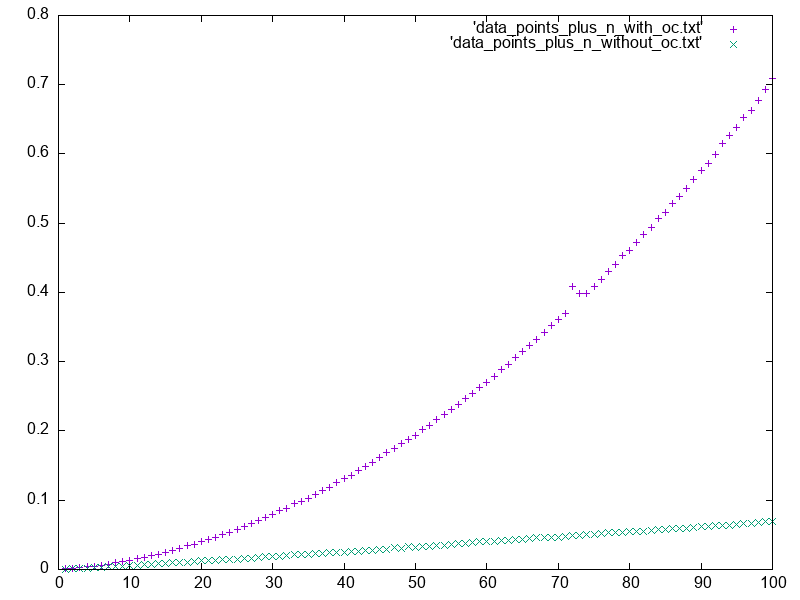
\includegraphics[width=10cm,height=8cm]{plot_example}
  \caption{The graph for the addition query showing the dependency of total time (in seconds) of the search for the query \lstinline|plus$^o$ $\,$ $\overline{n}$ $\,$ $\overline{m}$ $\,$ $r^?$| on the value of $n$ with a fixed $m$. Purple dots show the time for the case when occurs checks are performed, green dots~--- for the case when they are not performed. }
  \label{fig:plot_example}
\end{figure}

To check how well our estimates correspond to the reality we implemented a simple embedding of \mK into \textsc{OCaml} and measured the time of the search for the example queries,
building graphs for the time vs. parameters in the estimated complexity (distinct plot for each parameter).~\footnote{The implementation and the results of the measuring can be found at \url{https://www.dropbox.com/sh/ciceovnogkeeibz/AAAoclpTSDeY3OMagOBJHNiSa}} The referenced embedding follows the standard \textsc{microKanren} implementation but with standard library maps for substitutions and with possibility to switch occurs check on and off.
For time measuring we used standard \textsc{OCaml} library \textsc{benchmark}. The precision we were able to achieve is rather limited, so the plots are not always smooth and can have
deviations (especially for small sizes of the input), but the overall trend is usually clear. Because of the problems with precision, for now we are able to adequately measure only the total
time of the search, with or without occurs check, so we are basically verifying only the \figureword~\ref{fig:examples_total_times}. 
The example of the resulting graph is shown in \figureword~\ref{fig:plot_example} (the time of addition of two numbers depending on the first argument). The character of a time dependency function
is not always visible from the graph (when the degree of the polynomial is greater than one), but after studying each graph individually (for example, by placing the plot between two polynomials of the same degree) we are reasonably convinced that all the complexity estimates from the \figureword~\ref{fig:examples_total_times} are confirmed.


\section{Conclusion}

We presented a first attempt to build a theory which would allow one to calculate an adequate worst-case time
complexity estimations for relational programs in \mK. While our research is not completed the results still
allow to explain some observable phenomena in some relational programs behavior.

As the directions for future research we can mention relaxing the requirements which we put on
terms and substitutions in order to provide an accurate unification time estimations. It would be also
interesting to come up with an automated (or semi-automated) procedure to deduce the complexity
estimations in a symbolic forms by making use of symbolic execution model presened in Section~\ref{sec:symbolic}.

%%
%% The acknowledgments section is defined using the "acks" environment
%% (and NOT an unnumbered section). This ensures the proper
%% identification of the section in the article metadata, and the
%% consistent spelling of the heading.
\begin{acks}

\end{acks}

%%
%% The next two lines define the bibliography style to be used, and
%% the bibliography file.
\bibliographystyle{ACM-Reference-Format}
\bibliography{main}

%%
%% If your work has an appendix, this is the place to put it.
\appendix

\end{document}
\endinput
%%
%% End of file `sample-acmlarge.tex'.
